\chapter{Конструкторский раздел}
На рисунках \ref{fig:s}, \ref{fig:bs} и \ref{fig:ss} приведены схемы алгоритмов поиска в словаре. На рисунке  \ref{fig:seg} приведён алгоритм сегментирования для поиска по сегментам.

\begin{figure}[H]
	\centering
	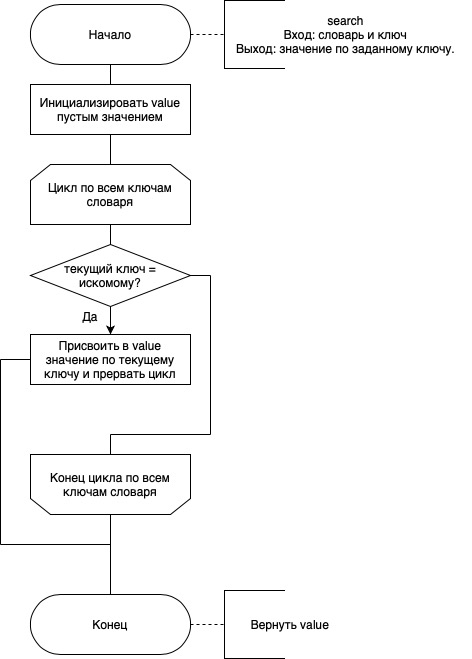
\includegraphics[scale=0.57]{inc/scheme-search.jpg}
	\caption{Схема алгоритма полного перебора.}
	\label{fig:s}
\end{figure}

\begin{figure}[H]
	\centering
	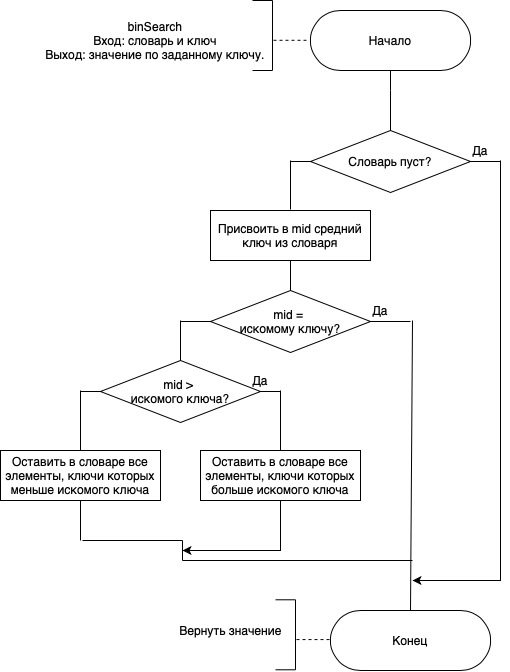
\includegraphics[scale=0.55]{inc/scheme-binSearch.jpg}
	\caption{Схема алгоритма двоичного поиска.}
	\label{fig:bs}
\end{figure}

\begin{figure}[H]
	\centering
	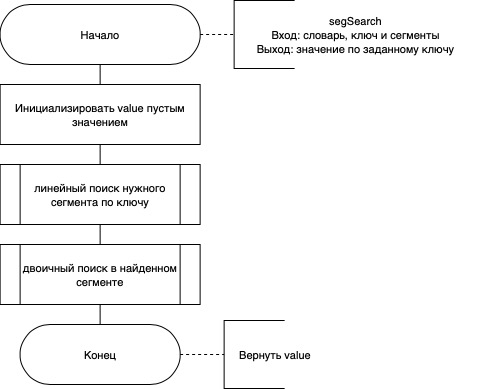
\includegraphics[scale=0.6]{inc/scheme-segSearch.jpg}
	\caption{Схема алгоритма поиска по сегментам.}
	\label{fig:ss}
\end{figure}

\begin{figure}[H]
	\centering
	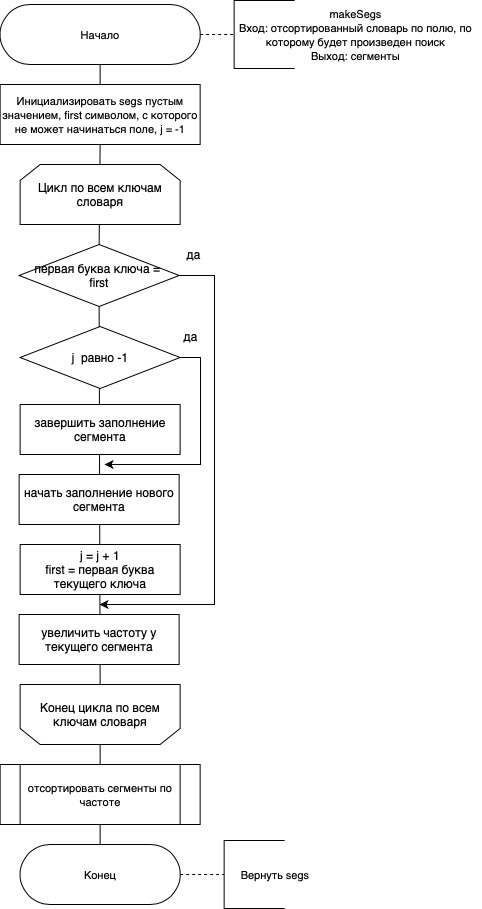
\includegraphics[scale=0.6]{inc/scheme-makeSegs.jpg}
	\caption{Схема алгоритма сегментирования.}
	\label{fig:seg}
\end{figure}

\section{Описание структур данных}
Для работы программы требуется ввести три основные структуры данных. Одна из них нужна для хранения записей, вторая -- для словаря, третья -- для описания информации о сегменте.

Каждая запись представляет собой структуру из двух полей. Первое отвечает за название страны, второе -- за количество случаев заболевания коронавирусом в этой стране.

Словарь -- массив структур типа записи, описанной выше.

Для описания сегмента требуется создать структуру, хранящую четыре поля:
\begin{itemize}
	\item start\_index -- индекс начала сегмента;
	\item end\_index -- индекс конца сегмента;
	\item letter -- буква, с которой начинаются названия стран в этом сегменте
	\item freq -- число записей в сегменте.
\end{itemize}

\section*{Вывод}

На основе теоретических данных, полученных из аналитического раздела, были построены схемы алгоритмов поиска в словаре. 

Также были определены структуры данных, которые нужны для реализации алгоритмов поиска.